\begin{figure}
\begin{center}

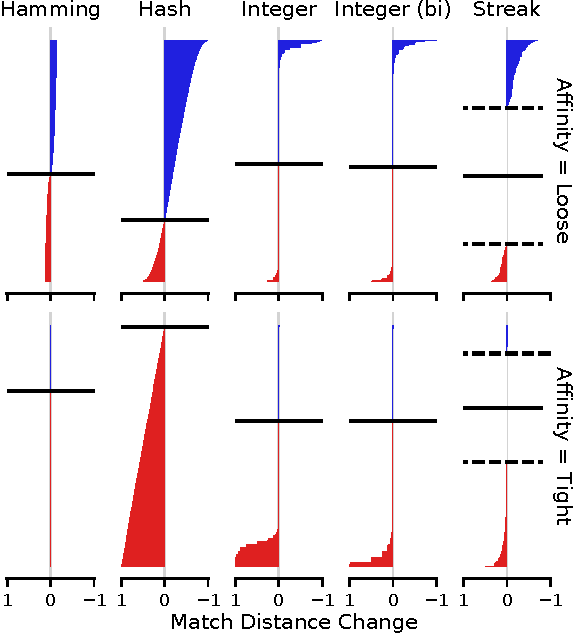
\includegraphics[width=\columnwidth]{mutational_step/bitweight=0dot5+seed=1+title=low-mutational-step+_data_hathash_hash=95a57768de56995a+_script_fullcat_hash=78f9965681c3a44b+ext=}
\caption{
Distributions of mutation effects on match distance for loosely matched (pre-mutation match distance $> 0.5$) and tightly matched (pre-mutation match distance $< 0.01$) tag pairs.
Each bar sliver represents a single independently sampled mutation on an independently sampled tag pair.
Mutations that increase affinity are colored blue and mutations that decrease affinity are colored red.
Solid lines indicate the median between mutations that increase match distance and mutations that decrease match distance.
Dashed lines demarcate the boundaries between non-neutral and perfectly-neutral mutations.
}
\label{fig:mutational_step}

\end{center}
\end{figure}
